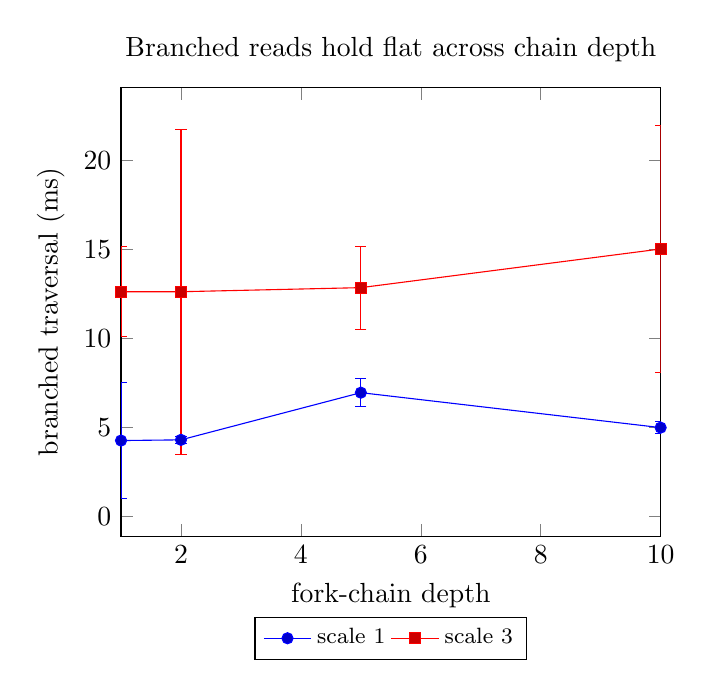
\begin{tikzpicture}
\begin{axis}[
  title={Branched reads hold flat across chain depth},
  xlabel={fork-chain depth},
  ylabel={branched traversal (ms)},
  xmin=1, xmax=10,
  legend style={at={(0.5,-0.18)},anchor=north,legend columns=-1,font=\footnotesize},
  error bars/y dir=both, error bars/y explicit,
]
  \addplot+[error bars/.cd,y explicit] coordinates {
    (1,4.272) +- (0,3.27)
    (2,4.312) +- (0,0.191)
    (5,6.96) +- (0,0.775)
    (10,4.998) +- (0,0.337)
  };
  \addlegendentry{scale 1}
  \addplot+[error bars/.cd,y explicit] coordinates {
    (1,12.621) +- (0,2.53)
    (2,12.624) +- (0,9.115)
    (5,12.853) +- (0,2.328)
    (10,15.023) +- (0,6.944)
  };
  \addlegendentry{scale 3}
\end{axis}
\end{tikzpicture}
{\footnotesize PRELIMINARY — non-reference hardware; medians of 5, bars show min/max. First readings, not reference figures (paper §5).\par}
